%% LyX 2.3.4.2 created this file.  For more info, see http://www.lyx.org/.
%% Do not edit unless you really know what you are doing.
\documentclass[english,dvipsnames,aspectratio=169]{beamer}
\usepackage{mathptmx}
\usepackage{eulervm}
\usepackage[T1]{fontenc}
\usepackage[latin9]{inputenc}
\usepackage{babel}
\usepackage{amstext}
\usepackage{amssymb}
\usepackage{graphicx}
\usepackage{ifthen}
\usepackage{colortbl}
\usepackage{xcolor}
\usepackage{algorithm2e}
\usepackage{xspace}
\usepackage{multirow}
\usepackage{tikz}
\usetikzlibrary{tikzmark}
\usetikzlibrary{calc}
\usepackage{pgfplots}
%\pgfplotsset{compat=1.17}
\usepackage{booktabs}
\usepackage{mathtools}




\ifx\hypersetup\undefined
  \AtBeginDocument{%
    \hypersetup{unicode=true,pdfusetitle,
 bookmarks=true,bookmarksnumbered=false,bookmarksopen=false,
 breaklinks=false,pdfborder={0 0 0},pdfborderstyle={},backref=false,colorlinks=true,
 allcolors=NYUPurple,urlcolor=LightPurple}
  }
\else
  \hypersetup{unicode=true,pdfusetitle,
 bookmarks=true,bookmarksnumbered=false,bookmarksopen=false,
 breaklinks=false,pdfborder={0 0 0},pdfborderstyle={},backref=false,colorlinks=true,
 allcolors=NYUPurple,urlcolor=LightPurple}
\fi

\makeatletter

%%%%%%%%%%%%%%%%%%%%%%%%%%%%%% LyX specific LaTeX commands.
%% Because html converters don't know tabularnewline
\providecommand{\tabularnewline}{\\}

%%%%%%%%%%%%%%%%%%%%%%%%%%%%%% Textclass specific LaTeX commands.
% this default might be overridden by plain title style
\newcommand\makebeamertitle{\frame{\maketitle}}%
% (ERT) argument for the TOC
\AtBeginDocument{%
  \let\origtableofcontents=\tableofcontents
  \def\tableofcontents{\@ifnextchar[{\origtableofcontents}{\gobbletableofcontents}}
  \def\gobbletableofcontents#1{\origtableofcontents}
}

%%%%%%%%%%%%%%%%%%%%%%%%%%%%%% User specified LaTeX commands.
\usetheme{CambridgeUS} 
\beamertemplatenavigationsymbolsempty


% Set Color ==============================
\definecolor{NYUPurple}{RGB}{87,6,140}
\definecolor{LightPurple}{RGB}{165,11,255}


\setbeamercolor{title}{fg=NYUPurple}
\setbeamercolor{frametitle}{fg=NYUPurple}

\setbeamercolor{background canvas}{fg=NYUPurple, bg=white}
\setbeamercolor{background}{fg=black, bg=NYUPurple}

\setbeamercolor{palette primary}{fg=black, bg=gray!30!white}
\setbeamercolor{palette secondary}{fg=black, bg=gray!20!white}
\setbeamercolor{palette tertiary}{fg=gray!20!white, bg=NYUPurple}

\setbeamertemplate{headline}{}
\setbeamerfont{itemize/enumerate body}{}
\setbeamerfont{itemize/enumerate subbody}{size=\normalsize}
\setbeamerfont{itemize/enumerate subsubbody}{size=\normalsize}


\setbeamercolor{parttitle}{fg=NYUPurple}
\setbeamercolor{sectiontitle}{fg=NYUPurple}
\setbeamercolor{sectionname}{fg=NYUPurple}
\setbeamercolor{section page}{fg=NYUPurple}
%\setbeamercolor{description item}{fg=NYUPurple}
%\setbeamercolor{block title}{fg=NYUPurple}

\setbeamertemplate{blocks}[rounded][shadow=false]
\setbeamercolor{block body}{bg=normal text.bg!90!NYUPurple}
\setbeamercolor{block title}{bg=NYUPurple!30, fg=NYUPurple}

\usepackage{pgfpages}
%\setbeameroption{show notes on second screen}
%\setbeamertemplate{note page}[default]

\AtBeginSection[]{
  \begin{frame}
  \vfill
  \centering
\setbeamercolor{section title}{fg=NYUPurple}
 \begin{beamercolorbox}[sep=8pt,center,shadow=true,rounded=true]{title}
    \usebeamerfont{title}\usebeamercolor[fg]{title}\insertsectionhead\par%
  \end{beamercolorbox}
  \vfill
  \end{frame}
}

\makeatother

\setlength{\parskip}{\medskipamount} 

\input ../macros

\begin{document}
\input ../rosenberg-macros

\title[DS-GA 1003]{Conclusion}
\author[Ravid Shwart Ziv]{Ravid Shwart Ziv}
\date{May 2, 2023}
\institute{CDS, NYU}

\makebeamertitle
\mode<article>{Just in article version}

\begin{frame}{Contents}
\tableofcontents{}
\end{frame}

\section{Summary of This Course}
\begin{frame}
{Rule-based approach}
\begin{center}
    \large{Code an algorithm}
\end{center}
\begin{figure}
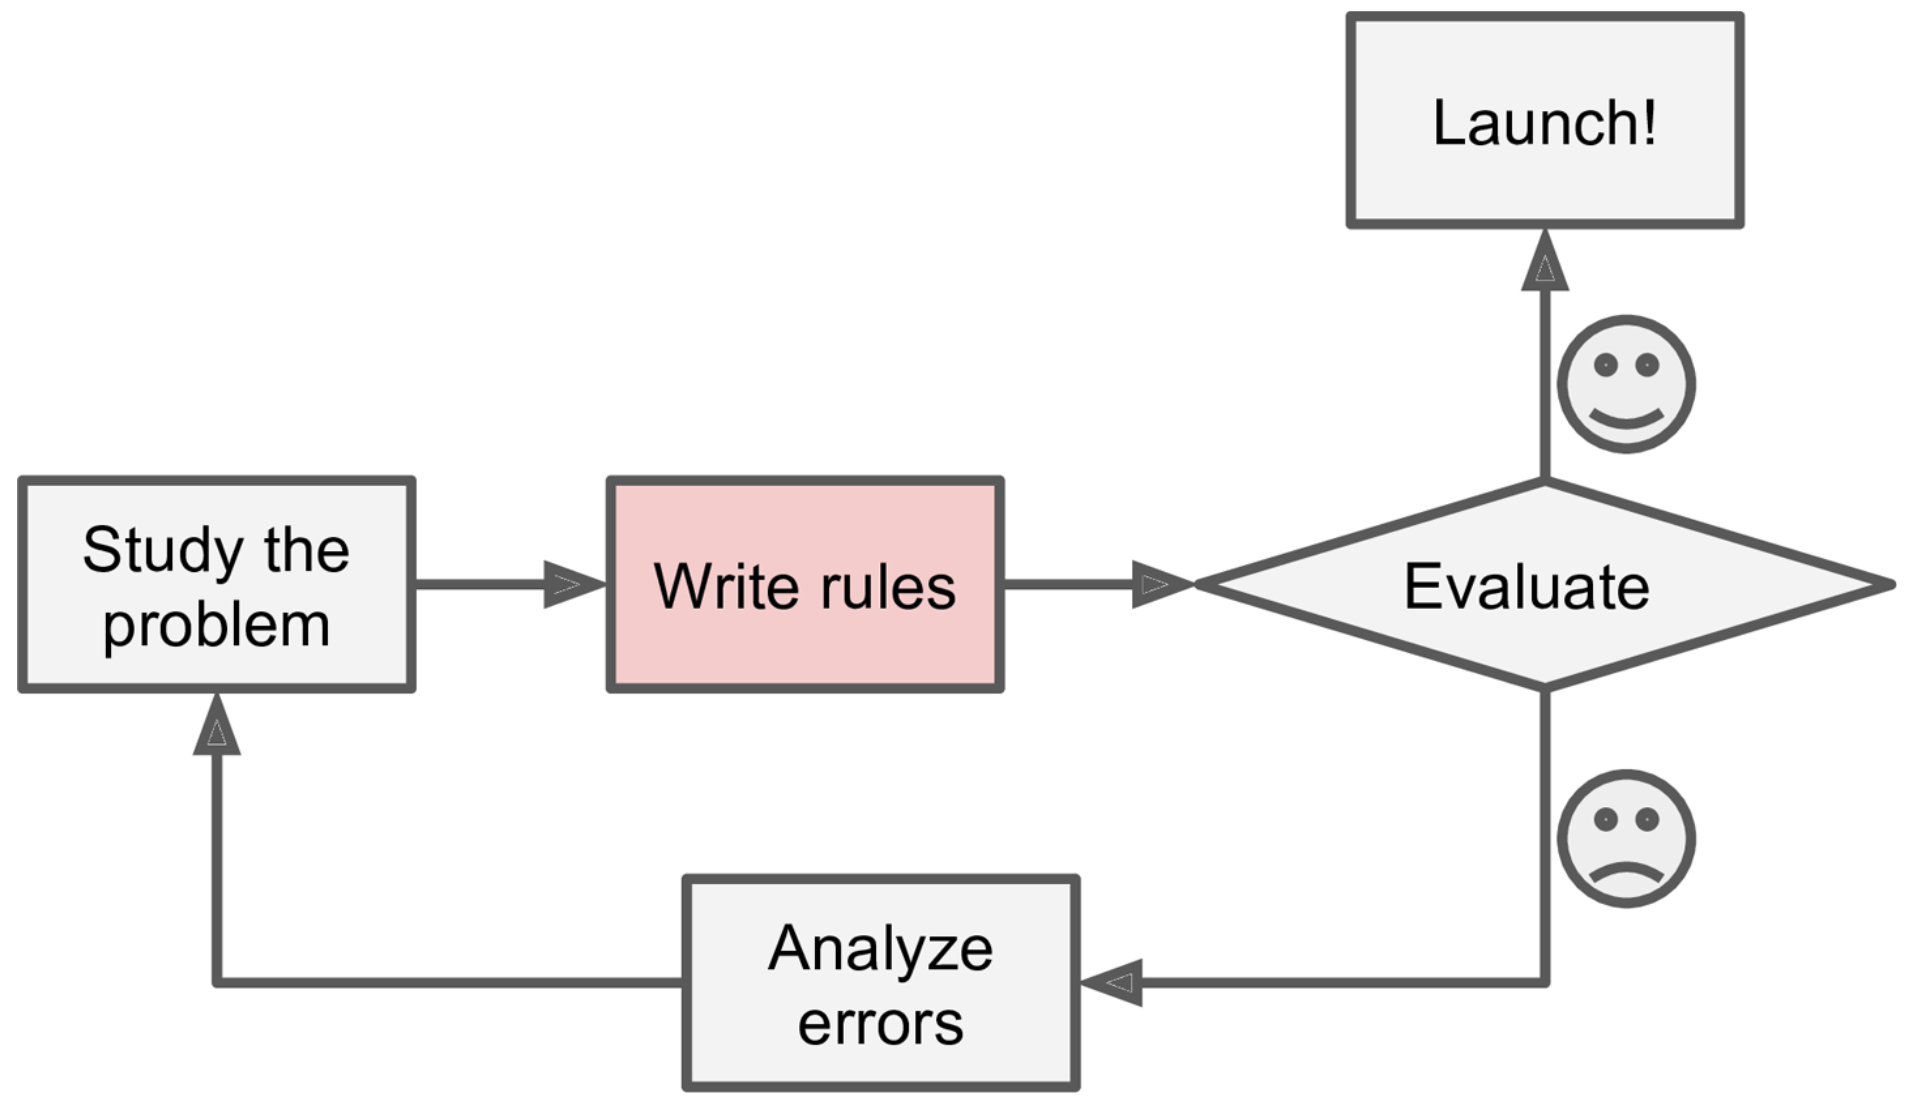
\includegraphics[width=0.7\textwidth]{figures/geron-fig1-1.png}
\end{figure}
    \note[item]{What is ML about? In AI, often times our goal is to build agents that can solve problems in place of humans. One approach is to write down what a human expert knows in some way (such as likely inference rules), so that machines can operate based on human knowledge. }
\note[item]{This is in fact the mainstream approach in the 80's. 
Note that the rules and inference are often more sophiscated than a list of if-then-else statements.
    It's still used now in some applications.
    It's interpretable, controllable, and easy to debug.}
\end{frame}

\begin{frame}
{Machine learning approach}
\begin{center}
    \large{Learn the algorithm from data}
\end{center}
\begin{figure}
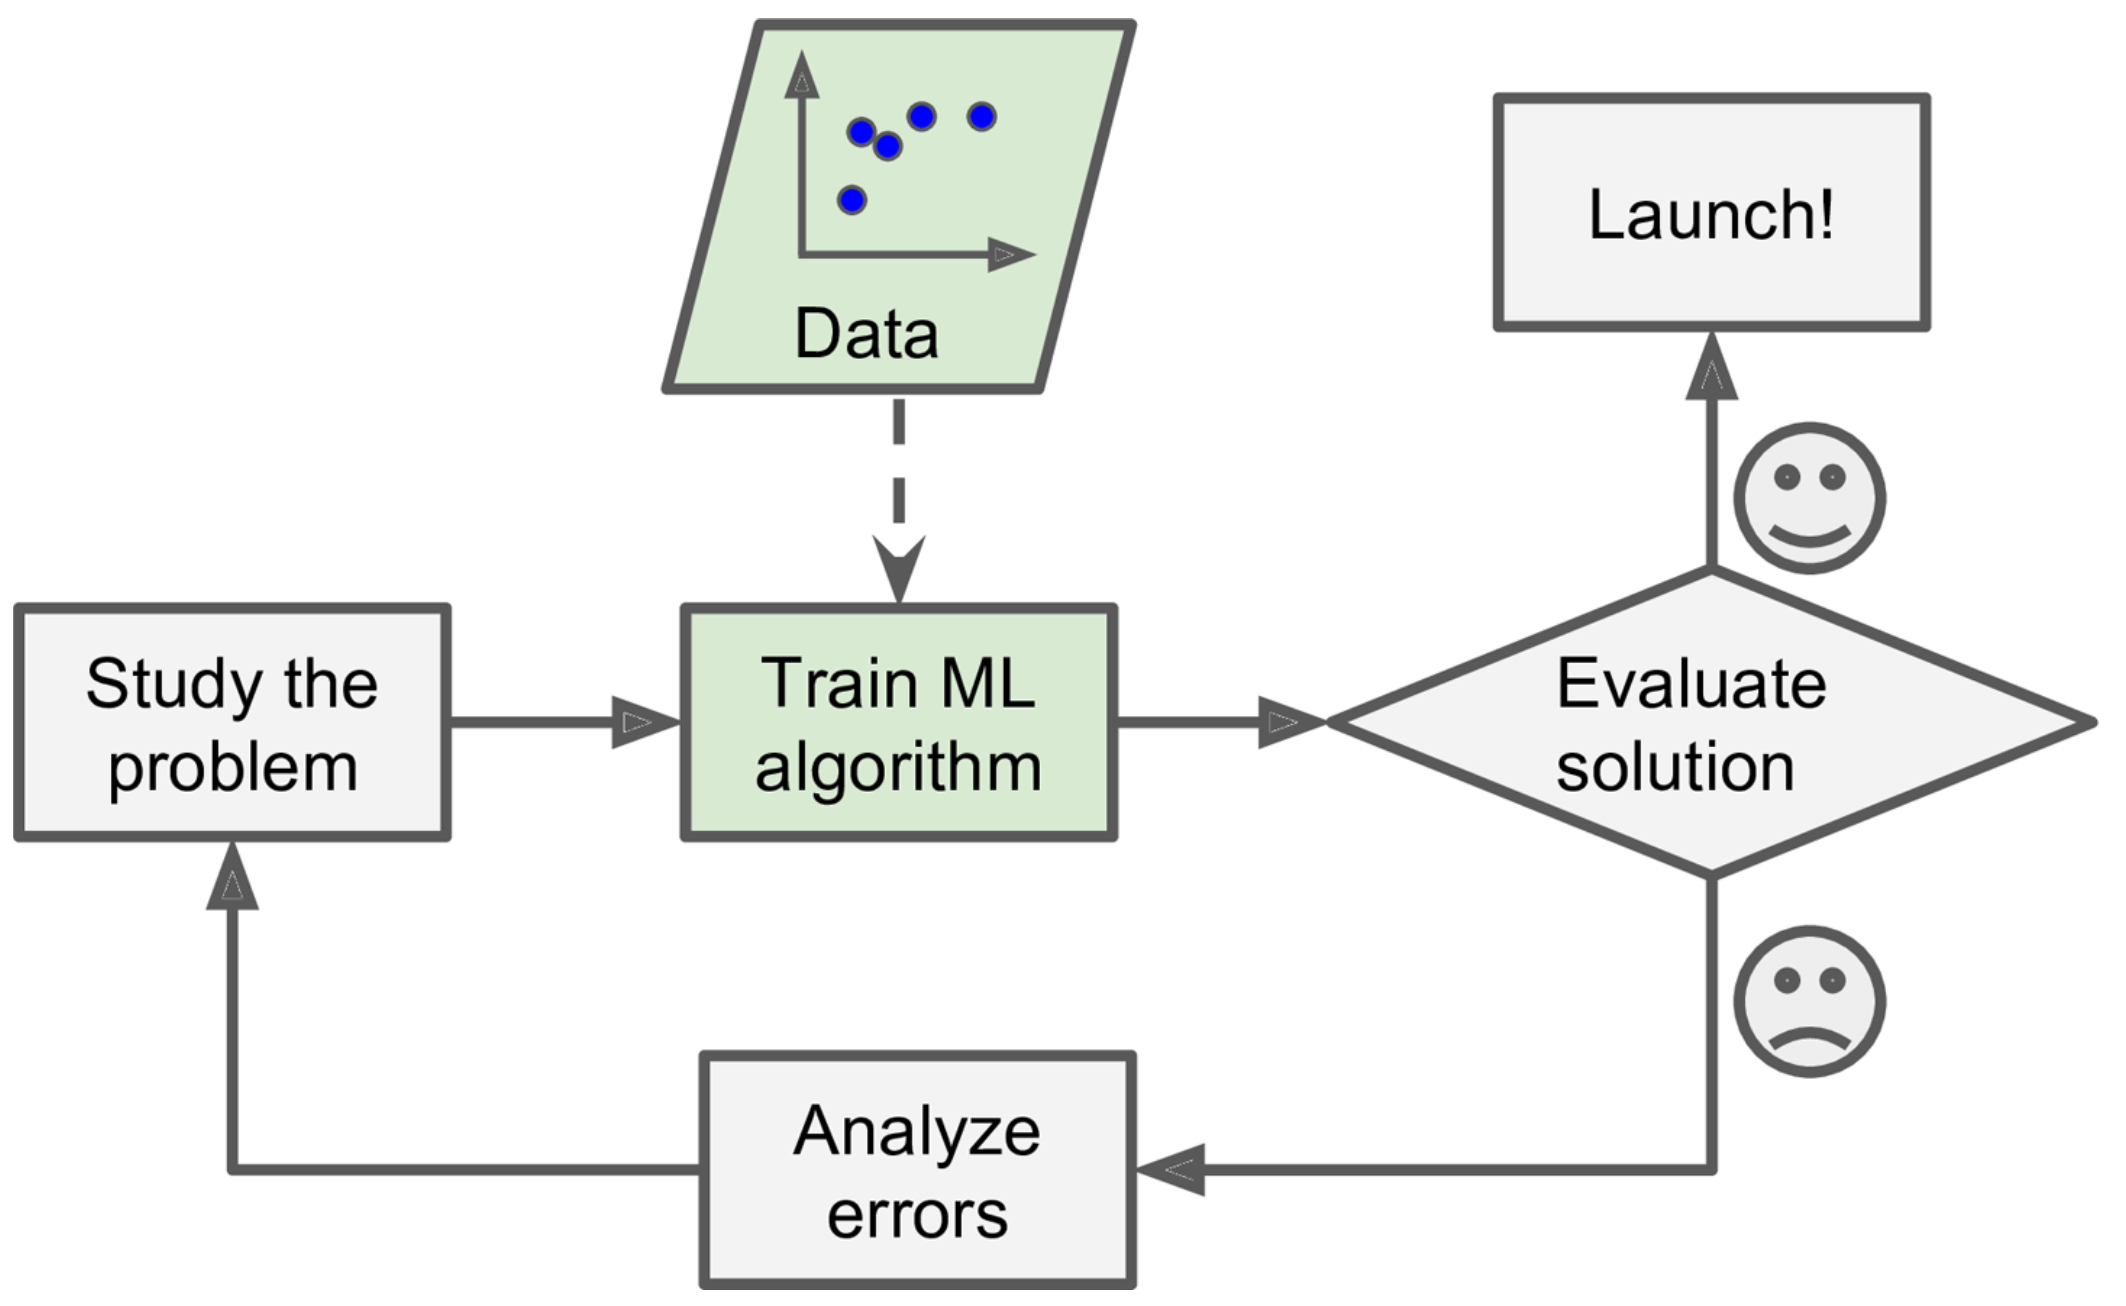
\includegraphics[width=0.7\textwidth]{figures/geron-fig1-2.png}
\end{figure}
\note[item]{However, in many cases, it's too complicated to encode all relevant knowledge for a task. There are also cases where it's much easier to demonstrate what the output should be instead of specifying the derivation of the output, \eg perception problems such as image recognition.}
\note[item]{ML is about learning the rules or the algorithms automatically from data.}
    \note[item]{That said, it is important to note that the system development pipeline is the same. The ML approach is not completely task-agnostic, we still need to study the task to incorporate any useful priors, look at the data to analyze errors, and iteratively improve the system.}
\end{frame}

\begin{frame}
{Machine learning vs rule-based approach}
\begin{center}
data $\xrightarrow{\mbox{learning algorithm}}$ model 
\end{center}
\begin{itemize}
\item Machine learning is the main driving force of modern AI.
\item Shift from specifying \emph{how to} solve the problem to \emph{what} the solution looks like. 
\item Promise: \emph{generalization} to unseen examples.
\end{itemize}
\note[item]{It's an important paradigm shift: instead of specifying how to solve the problem, we directly specify what the solution looks like, and let the machine figure out the how-to question.}
\note[item]{The promise made by the ML approach is that you can generalize to unseen data. And generalization has been one of the core questions in any ML algorithm.}
\note[item]{Of course now we should be aware of what generalization means. Most learning algorithms only guarantee generalization to unseen data from the same distribution. But the iid assumption almost never holds true in practice, which is one more reason for why you need to know the task at hand and how the data is generated.}
\end{frame}

\begin{frame}
{Typical machine learning recipe}
\begin{description}
\item[Model] A family of predictors that map from the input space to the action space:
\begin{align}
f(x; \theta) = a .
\end{align}
\item[Objective] Empirical risk minimization:
\begin{align}
\min_\theta \sum_{(x,y)\in \sD_{\text{train}}} L(x, y, \theta) .
\end{align}
\item[Algorithm] Stochastic gradient descent:
\begin{align}
\theta \leftarrow \theta - \alpha_t \nabla_\theta L(x, y, \theta) .
\end{align}
\end{description}
\note[item]{A typical ML recipe we've seen in this course consists of three steps.}
\end{frame}

\begin{frame}
{Models}
\begin{description}
\item[Linear] Perceptron, conditional probability models, SVMs
\item[Non-linear] Kernelized models, trees, basis function models, neural nets
\end{description}

\onslide<2->{
\begin{simpleblock}
{How to choose the model family?}
\begin{itemize}
\item Trade-offs:
\begin{itemize}
\item approximation error and estimation error (bias and variance),
\item accuracy and efficiency (during both training and inference).
\end{itemize}
\item Start from the task requirements, e.g. amount of data, computation resource
\end{itemize}
\end{simpleblock}
}
\note[item]{approximation error and estimation error: high capacity models such as neural nets give you lower approximation error, but the estimation error could be high thus you will need more data compared to other simpler models.}
\note[item]{accuracy and efficiency: you might have time constraints either during training or inference so you might prefer a simpler model even if the accuracy is lower.}
\note[item]{The suggestion is to start from the task requirements and choose your model accordingly.}
\end{frame}

\begin{frame}
{Objectives}
\begin{description}[Loss functions]
\item[Loss functions] How far off a prediction is from the target, e.g. 0-1 loss, margin-based loss, squared loss.
\onslide<2->{
\item[Risk] Expected loss - but expectation over what?
\begin{itemize}
\item Frequentist approach: expectation over data.
\begin{itemize}
\item Empirical risk minimization, \ie average loss on the training data.
\item Regularization: balance estimation error and generalization error.
\end{itemize}
\item Bayesian approach: expectation over parameters.
\begin{itemize}
\item Posterior: prior belief updated by observed data.
\item Bayes action minimizes the posterior risk.
}
\end{itemize}
\end{itemize}
\end{description}
\note[item]{The next core question in ML is how do we learn the parameters given a model.}
\note[item]{We covered many loss functions, and you should know when each of them is used.}
\note[item]{But loss functions depend on the unknown target, thus it's a random variable. We cannot use it to choose model parameters. So we have the notion of risk, or expected loss.}
\note[item]{If you want a point estimate, you can take the Bayes action which minimizes the posterior risk.}
\end{frame}

\begin{frame}
{Algorithms}
\begin{description}
\item[Learning] Find model parameters---often an optimization problem.
\begin{itemize}
\item (Stocahstic) (sub)gradient descent
\item Functional gradient descent (gradient boosting)
\item Convex vs non-convex objectives
\end{itemize}

\item[Inference] Answer questions given a learned model.
\begin{itemize}
\item Bayesian inference: compute various quantities given the posterior.
\item Dynamic programming: compute $\argmax$ in structured prediction.
\end{itemize}
\end{description}
\note[item]{Given the objective, we still need an algorithm to given us the optimal parameters.}
\note[item]{We refer to finding model params as ``learning'' and it's often an opt problem.}
\note[item]{Another topic we didn't discuss much in this course is inference. Once we find the parameters, how do we use the model to answer questions. For most model we covered, inference is trivial, \eg compute the function values. But there are cases where this can be challenging.}
\end{frame}

\section{Debugging Machine Learning Algorithms}

\begin{frame}
{Get it to work}
\begin{itemize}
\item This course provides you a \emph{toolbox}.
\item Motivate a tool from the problem.
\item Keep the solution as simple as possible.
\end{itemize}
\end{frame}

\begin{frame}
{How to start on a problem}
\begin{simpleblock}
{Given a task, \eg spam classification, how should we get started on the problem?}
\begin{itemize}
\item Approach 1: Analyze the problem/dataset, design the right features/models/objectives carefully, then implement the algorithm.
\item Approach 2: Implement a simple baseline quickly, see what's wrong with it and fix its problems.
\end{itemize}
\end{simpleblock}
\pause
\begin{center}
In practice, often an \emph{iterative process} with a mix of both approaches.
\end{center}
\let\thefootnote\relax\footnotetext{\tiny{Reference: Andrew Ng's advice on applying ML.}}
\end{frame}

\begin{frame}
{Practical scenario}
You build a logistic regression model with L2 regularization using bag-of-words features for the spam classification task. After running SGD for some iterations, validation error is 20\%. What do you do now?
\pause
\begin{itemize}
\item Get more data.
\item Better feature selection.
\item Try another optimizer.
\item Run SGD for longer.
\item Tune weights on the regularizer.
\item Try another model.
\item $\ldots$
\end{itemize}
\end{frame}

\begin{frame}
{Setting expectations on performance}
\begin{description}
\item[Lower bound] What's the dumbest/simplest predictor you can build?
\pause
\begin{itemize}
\item Always predict the majority class / target mean.
\item Decision/regression stump, \ie use only one feature.
\item Linear model (with regularization).
\end{itemize}
\pause

\item[Upper bound] What's the best performance you can get given the hypothesis space?
\pause
\begin{itemize}
\item Fit your model on the validation set without regularization, \ie cheating.
\end{itemize}
\end{description}
\end{frame}

\begin{frame}
{Overfitting vs underfitting}
\begin{description}
\item[Overfitting] Low bias, high variance
\item[Underfitting] High bias, low variance
\end{description}
\begin{figure}
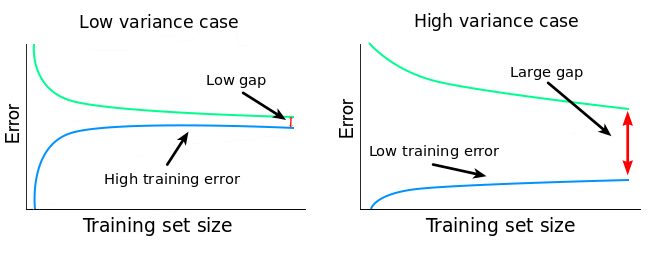
\includegraphics[width=0.8\textwidth]{figures/low_high_var.png}
\end{figure}
\let\thefootnote\relax\footnotetext{\tiny{Figure: \url{https://www.dataquest.io/blog/learning-curves-machine-learning/}.}}
\note[item]{How do we fix overfitting/underfitting?}
\end{frame}

\begin{frame}
{Fixes for high bias/variance}
\begin{description}[High variance]
\item[High variance]
\begin{itemize}
\item More data, bagging\\
\item Simpler feature, \eg remove rare words, L1 regularization
\item Simpler model, increase regularization strength
\end{itemize}

\item[High bias]
\begin{itemize}
\item Better feature, \eg n-grams
\item Increase model complexity, \eg neural nets
\item Reduce regularization strength
\end{itemize}
\end{description}
\end{frame}

\begin{frame}
{Optimization error}
\begin{simpleblock}
{Is there a problem with optimization?}
\onslide<2->{
\begin{itemize}
\item Look at the learning curve. Is the loss decreasing?
\item Verify initial loss, \eg $p(y\mid x)$ is a uniform distribution.
\item Add a cheating feature (\ie the label), does it achieve zero training error?
\end{itemize}
}
\end{simpleblock}

\onslide<3->{
\begin{simpleblock}
{Fixes}
\begin{itemize}
\item Tune the hyperparameters, \eg the learning rate.
\item Try another optimizer.
\end{itemize}
\end{simpleblock}
}
\end{frame}

\begin{frame}
{Error analysis}
\begin{description}
\item[Data] \textbf{Look at your data, but only the training/validation data!}
\begin{itemize}
\item Preprocessing errors, data corruption.
\item Label imbalance, noise.
\item Look at misclassified examples.
\item In general, print out as much information about the data as possible.
\end{itemize}
\pause

\item[Model] How much does each component help?
\begin{itemize}
\item \textbf{Ablation study}: change one thing at a time, \eg how much does the performance change if you add/remove the component?
\item \textbf{Oracle experiment}: use groundtruth information, \eg how much gain do you get if the output of the component is perfect?
\item Similar to how you would debug your code.
\end{itemize}
\end{description}
\note[item]{Oracle experiment. In our spam classification example, say you decide to first run a POS tagger, then take all the nouns as the feature of the classifier. Turns out it doesn't help much. Should you continue improving the POS tagger? An oracle experiment where you use groundtruth POS tags would tell you if it's worthwhile.}
\end{frame}

\begin{frame}
{Summary}
\begin{itemize}
\item Many things can go wrong: data, model, learning algorithm etc.
\item Fixes should be motivated by a problem identified from your analysis.
\item Verify that the fix actually fixes the problem it's intended to fix!
\item Be creative.
\end{itemize}
\end{frame}

\section{Next Steps}
\begin{frame}
{Other courses offered by CDS}
\begin{description}
\item[Foundations]
\begin{itemize}
\item DS-GA 1005 Inference and Representation
\item DS-GA 1008 Deep Learning
\item DS-GA 1013 Mathematical Tools for Data Science
\item DS-GA 3001 Special Topics in Data Science: Responsible Data Science
\end{itemize}
\item[Applications]
\begin{itemize}
\item DS-GA 1011 Natural Language Processing with Representation Learning
\item DS-GA 1012 Natural Language Understanding and Computational Semantics
\item DS-GA 3001 Special Topics in Data Science: Intro to Computer Vision
\item DS-GA 3001 Special Topics in Data Science: Computational Cognitive Modeling
\end{itemize}
\end{description}
\end{frame}

\begin{frame}
{Probabilistic graphical models}
\begin{columns}
\begin{column}{0.4\textwidth}\\
\begin{figure}
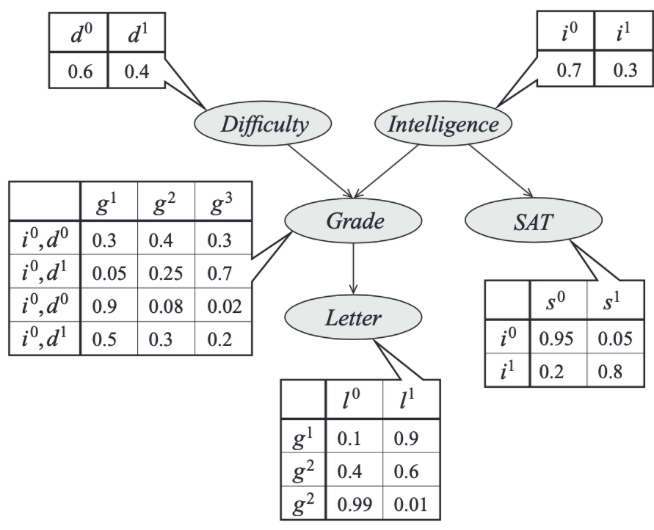
\includegraphics[width=1\textwidth]{figures/graphical-model}
\end{figure}
\end{column}

\begin{column}{0.6\textwidth}
\begin{itemize}
\item DS-GA 1005
\item Model: represent the world as a joint distribution of observed and unobserved variables.
\item Learning: estimate parameters of the distribution from data, \eg MLE.
\item Inference: compute posterior distribution of the latent variables.
\end{itemize}
\end{column}
\end{columns}
\end{frame}

\begin{frame}
{Deep learning}
\begin{columns}
\begin{column}{0.4\textwidth}\\
\begin{figure}
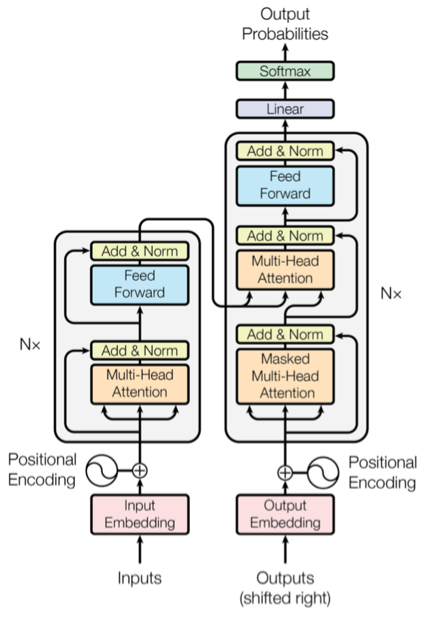
\includegraphics[scale=0.3]{figures/transformer}
\end{figure}
\end{column}

\begin{column}{0.6\textwidth}
\begin{itemize}
\item DS-GA 1008
\item Advanced neural network architectures: CNN, RNN, Seq2Seq, memory networks, Transformers etc.
\item Deep generative models: auto-encoders, GANs, energy-based models.
\item Representation learning: self-supervised learning.
\end{itemize}
\end{column}
\end{columns}
\end{frame}

\begin{frame}
{Ethics}
\begin{columns}
\begin{column}{0.4\textwidth}\\
\begin{figure}
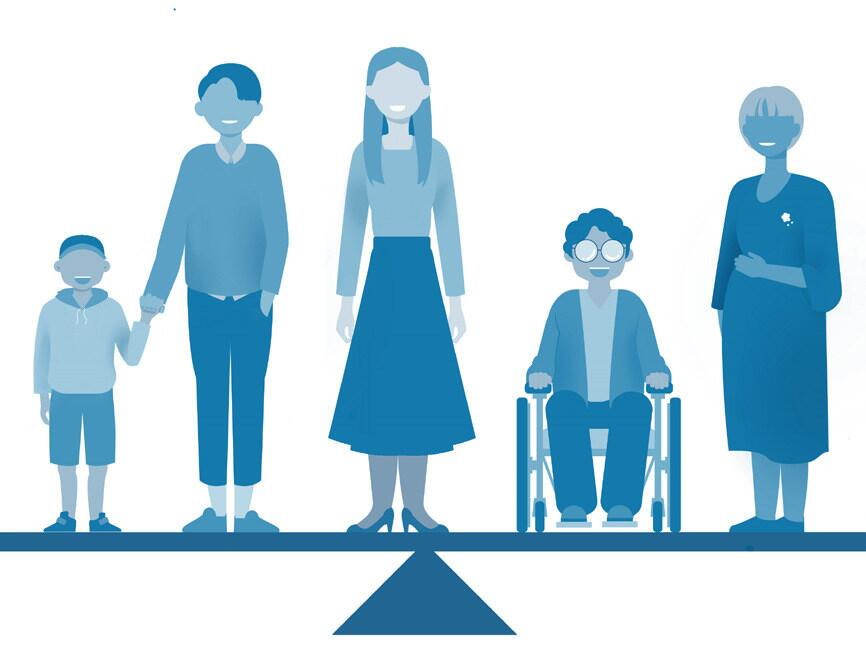
\includegraphics[scale=0.8]{figures/fairness}
\end{figure}
\end{column}

\begin{column}{0.6\textwidth}
\begin{itemize}
\item DS-GA 3001.009
\item Remember that the model we build will eventually impact \emph{people}.
\item Privacy: will the model/data leak user information?
\item Fairness: does the model ``discriminate'' a group of people?
\item Bias: does the model inherit bias in our society which generates the data?
\end{itemize}
\end{column}
\end{columns}
\end{frame}


\begin{frame}
{Language}
\begin{itemize}
\item DS-GA-10011, DS-GA-1012
\item Goal: teach computers to understand human languages.
\item Properties: discrete, compositional, ambiguous
\item Representation: how do we represent words, sentences, and documents?
\item Conditional sequence modeling: machine translation, summarization, dialogue etc.
\item Language understanding tasks: information extraction, entailment, question answering.
\end{itemize}
\note[item]{We should be careful when we say ``understand'' - what does that mean? Often it's easier to think about specific tasks.}
\end{frame}

\begin{frame}
{Vision}
\begin{itemize}
\item DS-GA 3001.005
\item Goal: teach computers to see the world as we see it.
\item Challenges:
\begin{itemize}
\item Low-level input: large amounts of raw pixels.
\item Variations of the same object: illumination, view point, occlusion, scale etc.
\end{itemize}
\item Tasks: object detection, video understanding, 3D vision etc.
\item Many related areas: medical imaging, robotics.
\end{itemize}
\end{frame}

\begin{frame}
{Cognitive modeling}
\begin{itemize}
\item DS-GA 1016
\item Goal: computational approaches to understanding human intelligence.
\item Why should machine learning care?
\begin{itemize}
\item Humans learn from a few examples---few shot learning.
\item Humans adapt to new concepts/environments quickly---transfer learning.
\item AI and cognitive science inform each other at both conceptual and technical levels.
\begin{itemize}
\item Reinforcement learning, neural nets, Bayesian modeling etc.
\end{itemize}
\end{itemize}
\end{itemize}
\end{frame}

\section{Machine Learning in the Wild}
\begin{frame}
{Google neural machine translation}
Approaching human performance [Wu+ 2016].
\begin{figure}
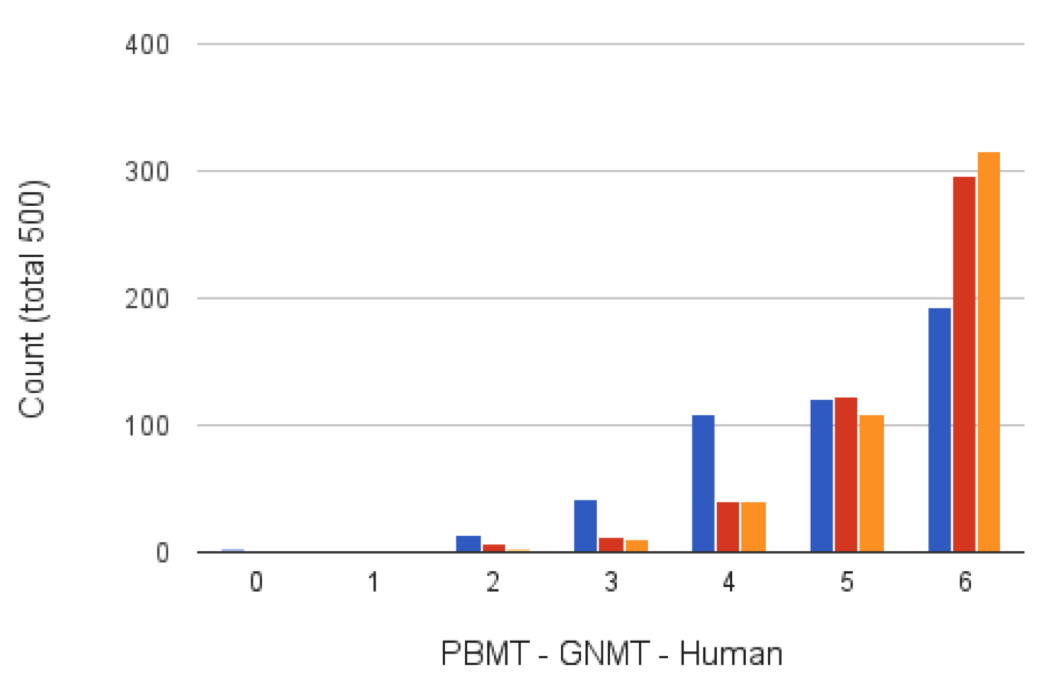
\includegraphics[height=0.7\textheight]{figures/gnmt}
\end{figure}
\end{frame}

\begin{frame}
{Gender bias in MT}
MT systems are prone to gender-biased translation errors [Stanovsky+ 2019].
\begin{figure}
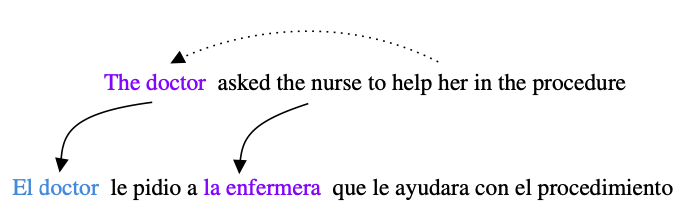
\includegraphics[scale=0.5]{figures/gender-bias-example}
\end{figure}
\end{frame}

\begin{frame}
{Object recognition}
Lower error rate than humans on ImageNet.
\begin{figure}
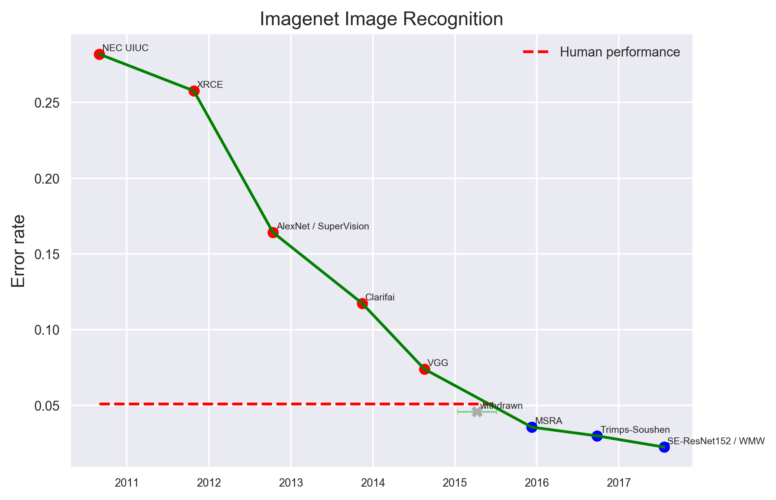
\includegraphics[height=0.7\textheight]{figures/imagenet}
\end{figure}
\let\thefootnote\relax\footnotetext{\tiny{Chart from Measuring the Progress of AI Research by EFF (CC BY-SA).}}
\end{frame}

\begin{frame}
{Adversarial examples}
Left: correct. Middle: added noise. Right: ostrich. [Szegedy+, 2013]
\begin{figure}
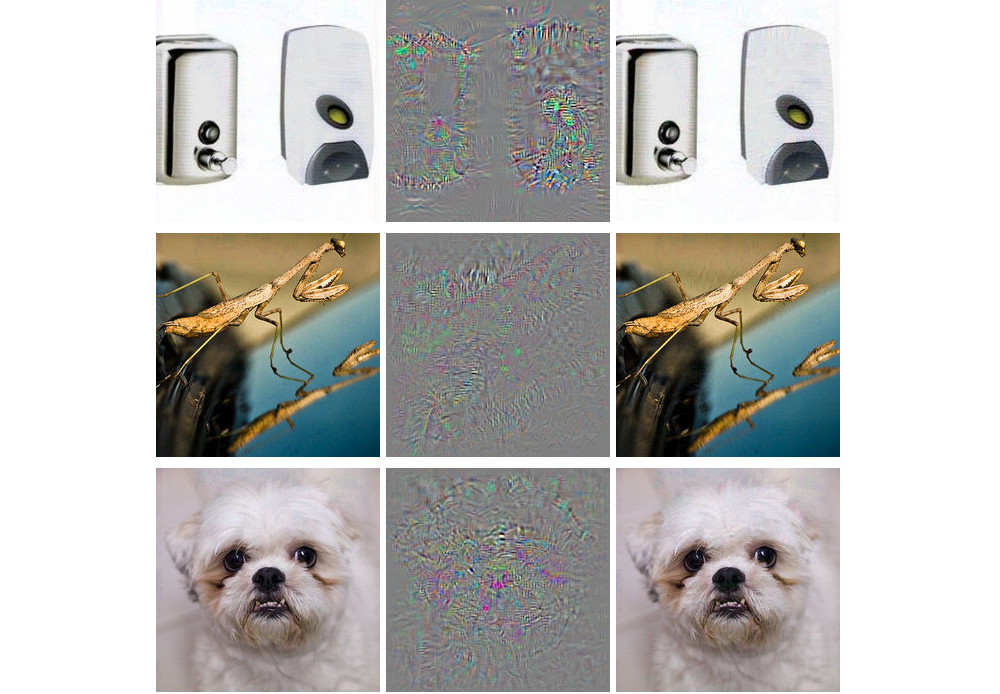
\includegraphics[height=0.7\textheight]{figures/adversarial-ostrich}
\end{figure}
\end{frame}

\begin{frame}
{Adversarial examples}
Left: real graffiti. Right: advesarial patches. [Eykholt+, 2018]
\begin{figure}
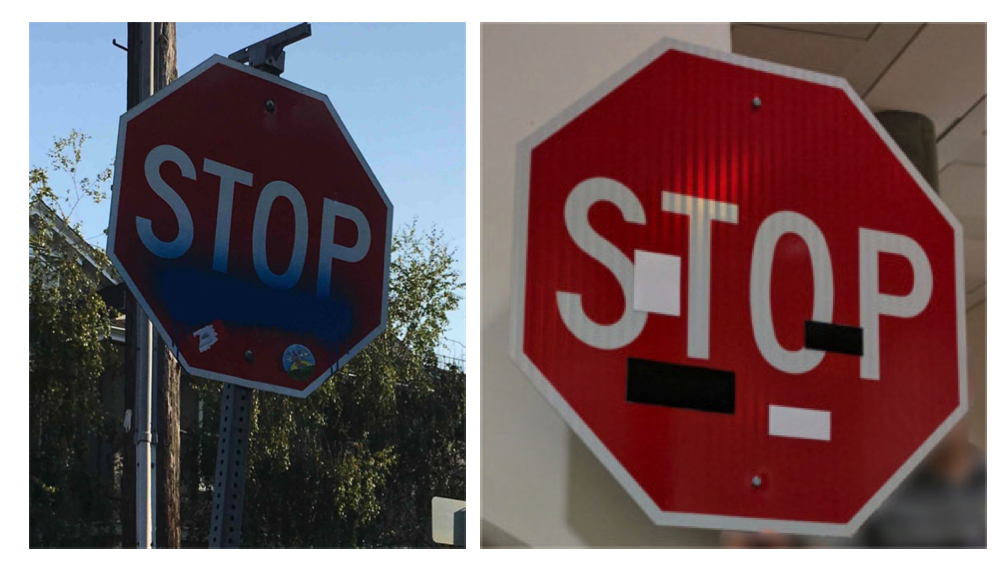
\includegraphics[height=0.7\textheight]{figures/stop-sign}
\end{figure}
\end{frame}

\begin{frame}
{Reinforcement learning}
Deepmind's AlphaGo beats the world's best human Go player.
\begin{figure}
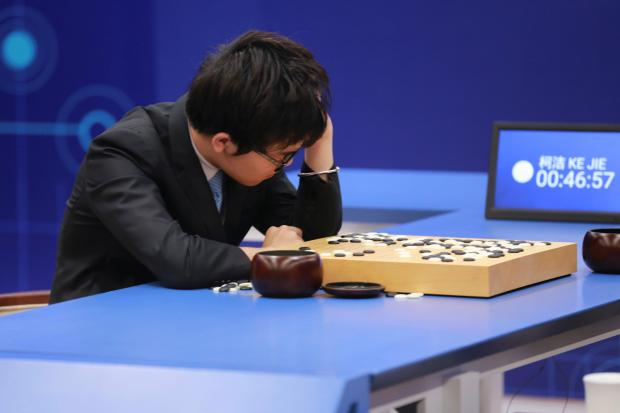
\includegraphics[height=0.7\textheight]{figures/alphago}
\end{figure}
\end{frame}

\begin{frame}
{Reward hacking}
Instead of finishing the course, agent learns to circle and attack target repeated despite bumping into other boats.

    \url{https://openai.com/blog/faulty-reward-functions/}
\begin{figure}
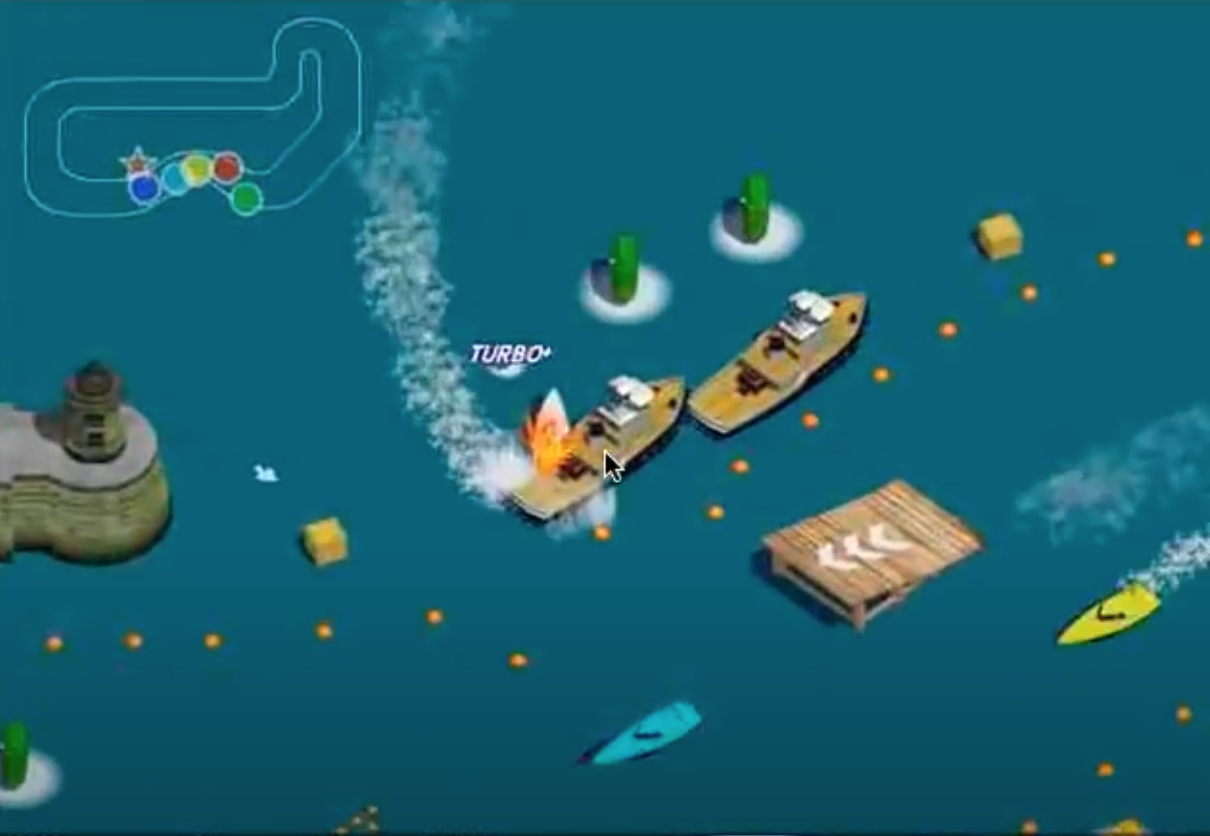
\includegraphics[height=0.6\textheight]{figures/boat}
\end{figure}
\end{frame}

\begin{frame}{Pretrained Models, Large Language Models}
\begin{itemize}
    \item Finish!
\end{itemize}
\end{frame}

\begin{frame}{Scaling of Parameters}
\end{frame}

\begin{frame}{Deep Learning}
\begin{itemize}
    \item Do we still need ML?
\end{itemize}
\end{frame}


\begin{frame}
    {Ethics of Machine Learning}
    Ensure that the behavior of machines towards human users is ethically acceptable.
    \begin{itemize}
         \item Bias and accountability in high-stake decisions
            \begin{itemize}
                \item Hiring, banking, legal, medical decisions etc.
            \end{itemize}
        \item Unintended, long-term influences
            \begin{itemize}
                \item Chat bots, recommender systems etc.
                \item Addiction, mental health etc.
            \end{itemize}
        \item Fairness: the system works well for a specific group of users
        \item Privacy: access to (private) data generated by users
        \item AI safety: Potential risks of AI taking over humanity?
    \end{itemize}
\end{frame}

\begin{frame}
{Food for thought}
\begin{itemize}
\item Should the learning objective be maximizing accuracy?
\item Who is responsible and what to do when ML systems go wrong?
\item How do we factor in humans when designing models?
\end{itemize}
% \vspace{3em}
% \begin{center}
% \emph{Thank you!}
% \end{center}
\end{frame}

\begin{frame}
\end{frame}

\end{document}
